% ===============================================================================
% = LaTeX Beamer Template des Arbeitsbereichs Sicherheit in verteilten Systemem
% = (c) 2016 Prof. Dr. Hannes Federrath, Uni Hamburg, Fachbereich Informatik
% = https://svs.informatik.uni-hamburg.de
% =
% = Weitgehend in Übereinstimmung mit dem Corporate Design 2016 der UHH:
% = https://www.uni-hamburg.de/beschaeftigtenportal/services/oeffentlichkeitsarbeit/corporate-design.html
% = 
% ===============================================================================
%
\documentclass[t,aspectratio=169]{beamer} 
% Option t              Place text of slides at the (vertical) top of the slides.
% Option handout        Ein PDF ohne Pausen und Overlayeffekte erzeugen.
% Option aspectratio=43 169 => 16:9, 1610 => 16:10, 43 => 4:3
\usepackage[utf8]{inputenc}
\usepackage[ngerman]{babel}
\usepackage{graphicx,xcolor}
\usepackage{tikz}
\usetikzlibrary{positioning}
\usetikzlibrary{calc}
\usepackage[T1]{fontenc} % 8-Bit-Zeichen; ermöglicht korrektes Kopieren von Umlauten aus dem pdf 
\bibliography{bib}
\bibliographystyle{ieee}
\usepackage{biblatex}
\addbibresource{bib.bib}

% SVS-Theme benutzen
\usetheme{svs2021}

% =============================
% = Ab hier Inhalte ändern... 
% =============================

\title{Introduction to Secure Multi-Party Computation (SMPC)}
% \subtitle{Ein Vorschlag}
\author[]{Jonas Müller, Rebekka Schnoor}
% \institute[Uni Hamburg]{Universität Hamburg · Fachbereich Informatik}
\date{30.04.2026} % Ausblenden geht mit leerem Inhalt: \date{}
% \titlegraphic{\uhhlogo} % Logo für Titelseite, UHH-Logo ist Standard
\eventlocation{Master Project Seminar Data Protection and Data Security, Hamburg, 30. April 2026} % rechts oben auf Titelseite

\begin{document}

\begin{frame}
	% Die Titelseite erscheint nach erneutem Übersetzen korrekt.
	\maketitle
\end{frame}

\begin{frame}
	\frametitle{Agenda}
	% Die Gliederung erscheint nach erneutem Übersetzen korrekt.
	% Die Gliederung wird im Dokument fortlaufend durch \section{} und \subsection{} definiert. Die Folien selbst haben keinen Einfluss auf die Gliederung.
	\tableofcontents
	% Hinweis: Das pandoc-Template benutzt \tableofcontents[hideallsubsections] zur Erzeugung einer Gliederung. Daher werden in der Markdown-Version nur die Überschriften der ersten Ebene (#) im Inhaltsverzeichnis angezeigt. Die normalerweise bei Verwendung von pandoc erzeugten Zwischenfolien für jede Überschrift der ersten Ebene werden im Theme unterdrückt. 
\end{frame}
\section{Motivation}
\section{Requirements}
\section{Algorithms}
\section{Limitations}

\begin{frame}{Motivation}
\begin{columns}[T]
    \begin{column} {0.4 \textwidth}
    \vspace{1.5cm}
    \begin{itemize}
        \item [] Several parties aim to compute a shared outcome without disclosing their private inputs.   
        \item[] \textcolor{gray}{Example: Obtain the average salary within a team without disclosing the individual salaries}
    \end{itemize}
    \end{column}
    \begin{column} {0.6\textwidth}
        \begin{figure}
    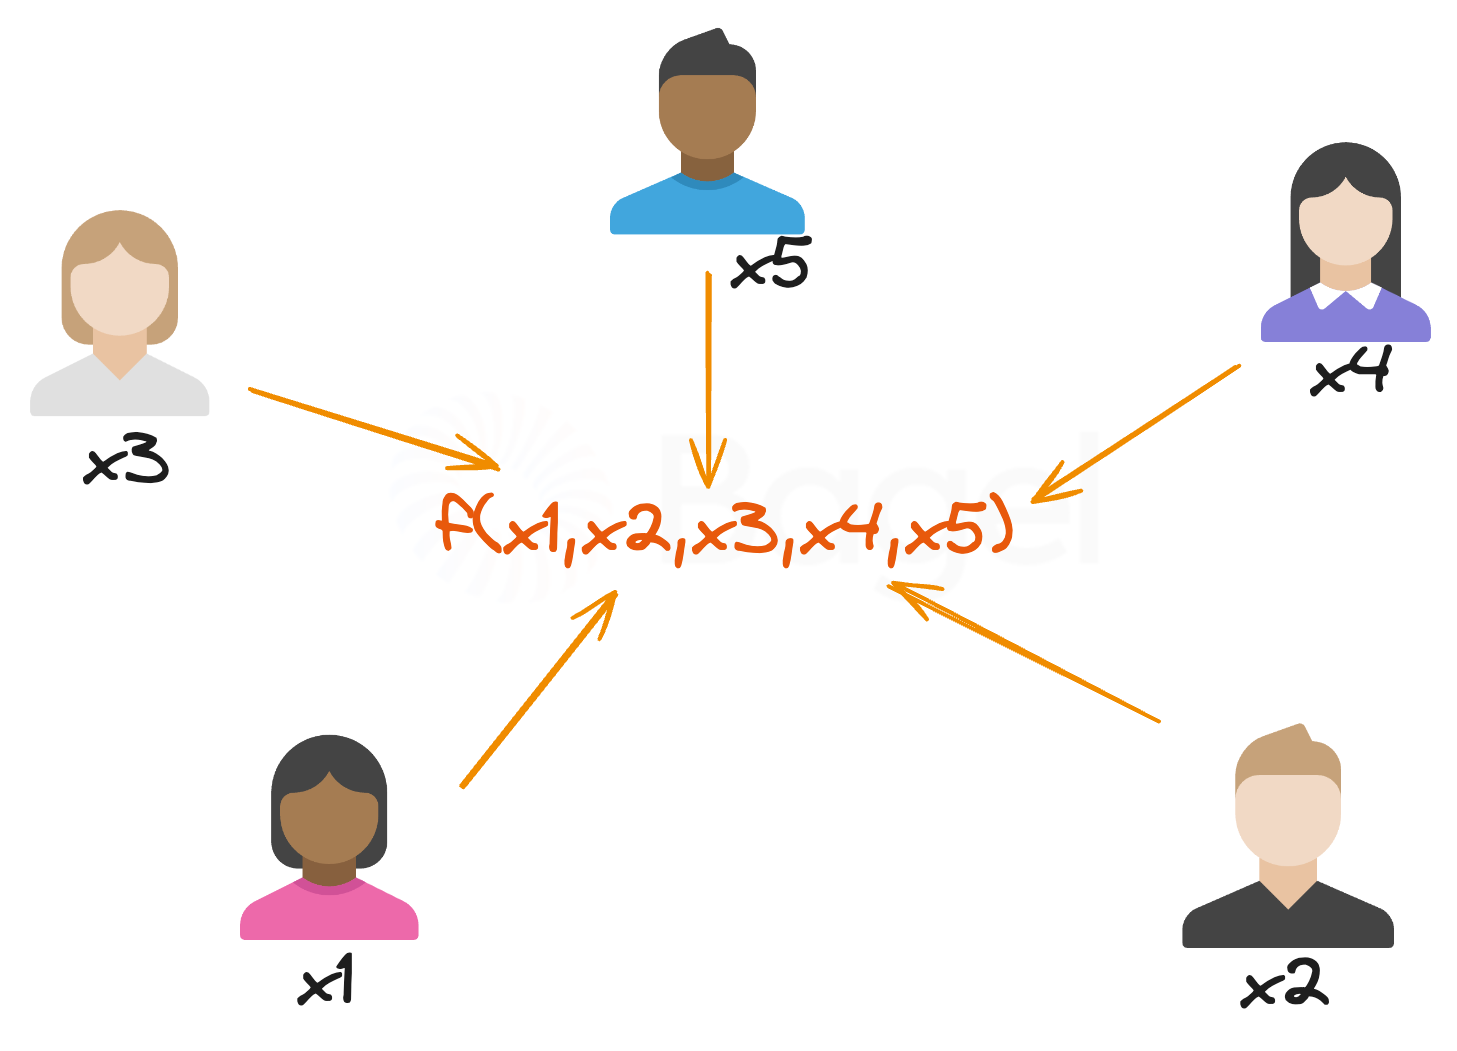
\includegraphics[width=\linewidth]{smpc.png}
\end{figure}
    \end{column}
    \end{columns}


\end{frame}

\begin{frame}{Requirements}
    \begin{enumerate}
        \item Privacy
        \begin{itemize}
            \item[] No party can learn any information about the others besides the output
        \end{itemize}
        \item Correctness
                \begin{itemize}
            \item[] Each party is guaranteed to get the correct output at the end of the computation
        \end{itemize}
        \item Independence of inputs
                \begin{itemize}
            \item[] Each party can independently choose their input
        \end{itemize}
        \item Guaranteed output delivery
                \begin{itemize}
            \item[] Malicious parties cannot block honest parties from obtaining the output
        \end{itemize}
        \item Fairness
                \begin{itemize}
            \item[] All parties get access to the output
        \end{itemize}
    \end{enumerate}
\end{frame}

\begin{frame}{Oblivious Transfer}
\begin{columns}[T]
    \begin{column} {0.5\textwidth}
        \begin{itemize}
            \item[] Fundamental building block for many SMPC protocols
            \begin{itemize}
            \item Transfer one message from a set of n messages
            \item Sender does not know which message was chosen
            \item Receiver learns only the chosen message
            \end{itemize}
            \item[] Implementation using asymmetric cryptography
        \end{itemize}
        
    \end{column}

    \begin{column} {0.5\textwidth}
        \begin{centering}
            \begin{tikzpicture}[
                node distance=1.2cm,   
                every node/.style={font=\small},
                circ/.style={circle, draw, minimum size=1cm, align=center}, 
                func/.style={rectangle, draw, minimum width=2.4cm, minimum height=1cm, align=center}
            ]
            % Nodes
            \node[circ] (msgs) {\shortstack{$W^1_E,$ \\ $\ldots,$ \\ $ m_n$}};
            \node[circ, right=2.2cm of msgs] (bit) {$b$};
            \node[func, below=1.2cm of $(msgs)!0.5!(bit)$] (fbox) {$f(W^1_E, ..., m_n, b)$};
            \node[circ, below=1.2cm of fbox] (out) {$m_b$};
            % Arrows
            \draw[->] (msgs) -- (fbox);
            \draw[->] (bit) -- (fbox);
            \draw[->] (fbox) -- (out);
            
            \end{tikzpicture}
        \end{centering}
    \end{column}
\end{columns}
\end{frame}

\begin{frame}{Additive secret sharing \cite{geeksforgeeks_smpc}}
\begin{columns}
    \begin{column} {0.3\textwidth}
    \begin{alertblock} {Roles}
        $n$ participants
    \end{alertblock}
        \begin{alertblock} {Threat model}
            semi-honest \\ less than $n-1$ parties collude \\
            Extension to malicious adversaries: MAC
        \end{alertblock}
    \end{column}
    \begin{column} {0.7\textwidth}

        \begin{enumerate}
            \item Each party splits their data $d_i$ into $n$ parts $s_1,...,s_n$, such that $\sum_{j=1}^ns_j=d_i$ and sends $s_i$ to party $i$
            \item Each party computes the sum of the received values and shares it with the other parties
            \item Each party computes the sum of the received sums, which is equivalent to the sum of all $d_i$
        \end{enumerate}
        \end{column}
    \end{columns}
\end{frame}
\begin{frame}{Yao's garbled circuits: Secure 2-party computation \cite{giapppp_isogeny_nodate}}

\begin{columns}[T]
\begin{column} {0.2\textwidth}
    \begin{alertblock}{Roles} \\ Garbler G and \\ Evaluator E
    \end{alertblock}
    
    \begin{alertblock}{Threat Model} semi-honest
    \end{alertblock}
\end{column}
\begin{column}{0.8\textwidth}
     \begin{enumerate}
     \item G picks random labels $W^0_G$, $W^1_G$, $W^0_E$, $W^1_E$ corresponding to $g=0, g=1, e=0, e=1$.
     \item G creates the permuted garbled output and shares with E
     \item G knows $g$ and therefore transmits $W^g_G$
     \item Access to more than one input-output-relation would reveal information about $g$. To ensure that G doesn't learn $e$ and E only learns one ciphertext, $W^e_E$ is transmitted using Oblivious Transfer
     \item E can now decrypt the output and shares it with G
 \end{enumerate}
\end{column}
\end{columns}
\begin{figure}
    \centering
    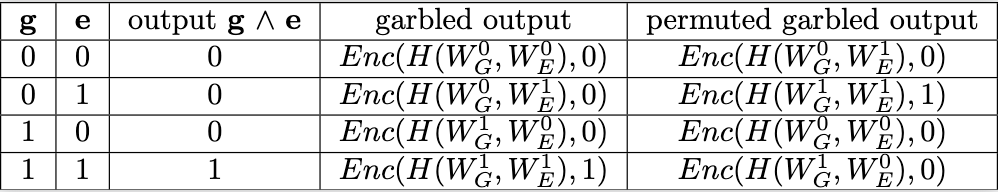
\includegraphics[width=0.75\linewidth]{img/grabled_and.png}
\end{figure}

\end{frame}

\begin{frame}{Limitations}
\vspace*{\fill}
\begin{itemize}
    \item Computational overhead
    \begin{itemize}
        \item[] $\xrightarrow{}$ Limited applicability on IoT or mobile devices
    \end{itemize}
    \item High communication costs / latency
    \begin{itemize}
        \item[] $\xrightarrow{}$ Infeasible for real-time applications
        \item[] $\xrightarrow{}$ Scalability issues
    \end{itemize}
    \item Vulnerable to dishonest majority scenarios
    \item Strict data structure requirements
\end{itemize}
\vspace*{\fill}
\end{frame}

\begin{frame}{1-2 Oblivious Transfer \cite{chou2015simplest}}
    \begin{itemize}
  \item Ginny holds two messages $W^0_E$, $W^1_E$ and wants Evan to learn exactly one of them.
  \item She generates an RSA key pair $(N, e, d)$ and chooses two random values $x_0, x_1$.  
        She sends $(N, e, x_0, x_1)$ to Evan.
  \item Evan selects his input $e \in \{0,1\}$ and picks $x_e$.  
        He samples a random value $k$ and computes
\[
            v = (x_b + k^e) \bmod N.
        \]
        He sends $v$ to Ginny.
  \item Ginny computes
\[
            k_0 = (v - x_0)^d \bmod N, \qquad
            k_1 = (v - x_1)^d \bmod N.
        \]
      Exactly one of these equals Evan's $k$; the other is pseudorandom from Evan's perspective.
 \end{itemize}

 \end{frame}
 \begin{frame}{1-2 Oblivious Transfer \cite{chou2015simplest}}
\begin{itemize}

  \item Ginny masks her messages using the two keys:
\[
            W^0_E' = (W^0_E + k_0) \bmod N, \qquad
            W^1_E' = (W^1_E + k_1) \bmod N,
        \]
        and sends $(W^0_E', W^1_E')$ to Evan.
  \item Evan recovers his chosen message by computing
\[
            m_e = (m_e' - k) \bmod N.
        \]
        Without knowing $d$, he cannot derive the other key and thus cannot obtain $W^{1-e}_E$
\end{itemize}
\end{frame}

\begin{frame}{References}
    \printbibliography
\end{frame}
\end{document}